\section{Usability-Studie BYU 2019}

\subsection*{Allgemeines}
\begin{frame}
    \frametitle{Usability-Studie BYU 2019}

    \begin{itemize}
        \item Brigham Young Universität, Utah
        \item 2 unabhängige Studien
              \begin{enumerate}
                  \item zwei-wöchige Studie zur Nutzung der 2FA-Methode
                  \item Studie zur Einrichtung der verschiedenen Methoden
              \end{enumerate}
        \item Betrachtung von Zeit und Gebrauchstauglichkeit
    \end{itemize}

    \note{
        \ldots
    }

\end{frame}

\subsection{tagtägliche Nutzung}
\begin{frame}
    \frametitle{\currentsectionname}

    \begin{itemize}
        \item 73 Teilnehmer*innen
        \item 6 Gruppen \'{a} 12 Personen
        \item Einloggen in Online Banking-App
        \item Absolvieren von 12 Aufgaben innerhalb von zwei Wochen
    \end{itemize}

    \note{
        \begin{itemize}
            \item Behandelte 2FA Methoden und Kontrollgruppe ohne 2FA
                  \begin{itemize}
                      \item SMS
                      \item TOTP
                  \end{itemize}
            \item maximal eine Aufgabe pro Tag
            \item keine `remember me`-Funktion, sodass immer zweiter Faktor benutzt werden musste
        \end{itemize}
    }

\end{frame}

\begin{frame}
    \frametitle{Authentifizierungszeit}

    \begin{itemize}
        \item Zeit von erfolgreicher Eingabe des Passworts bis Authentifizierung
    \end{itemize}
    % tabellarische Darstellung
    % \pgfplotstabletypeset[col sep=comma,
    %     columns/2FA-Methode/.style={string type},
    % ]{data/authentication-time.csv}
    \begin{figure}[c]
        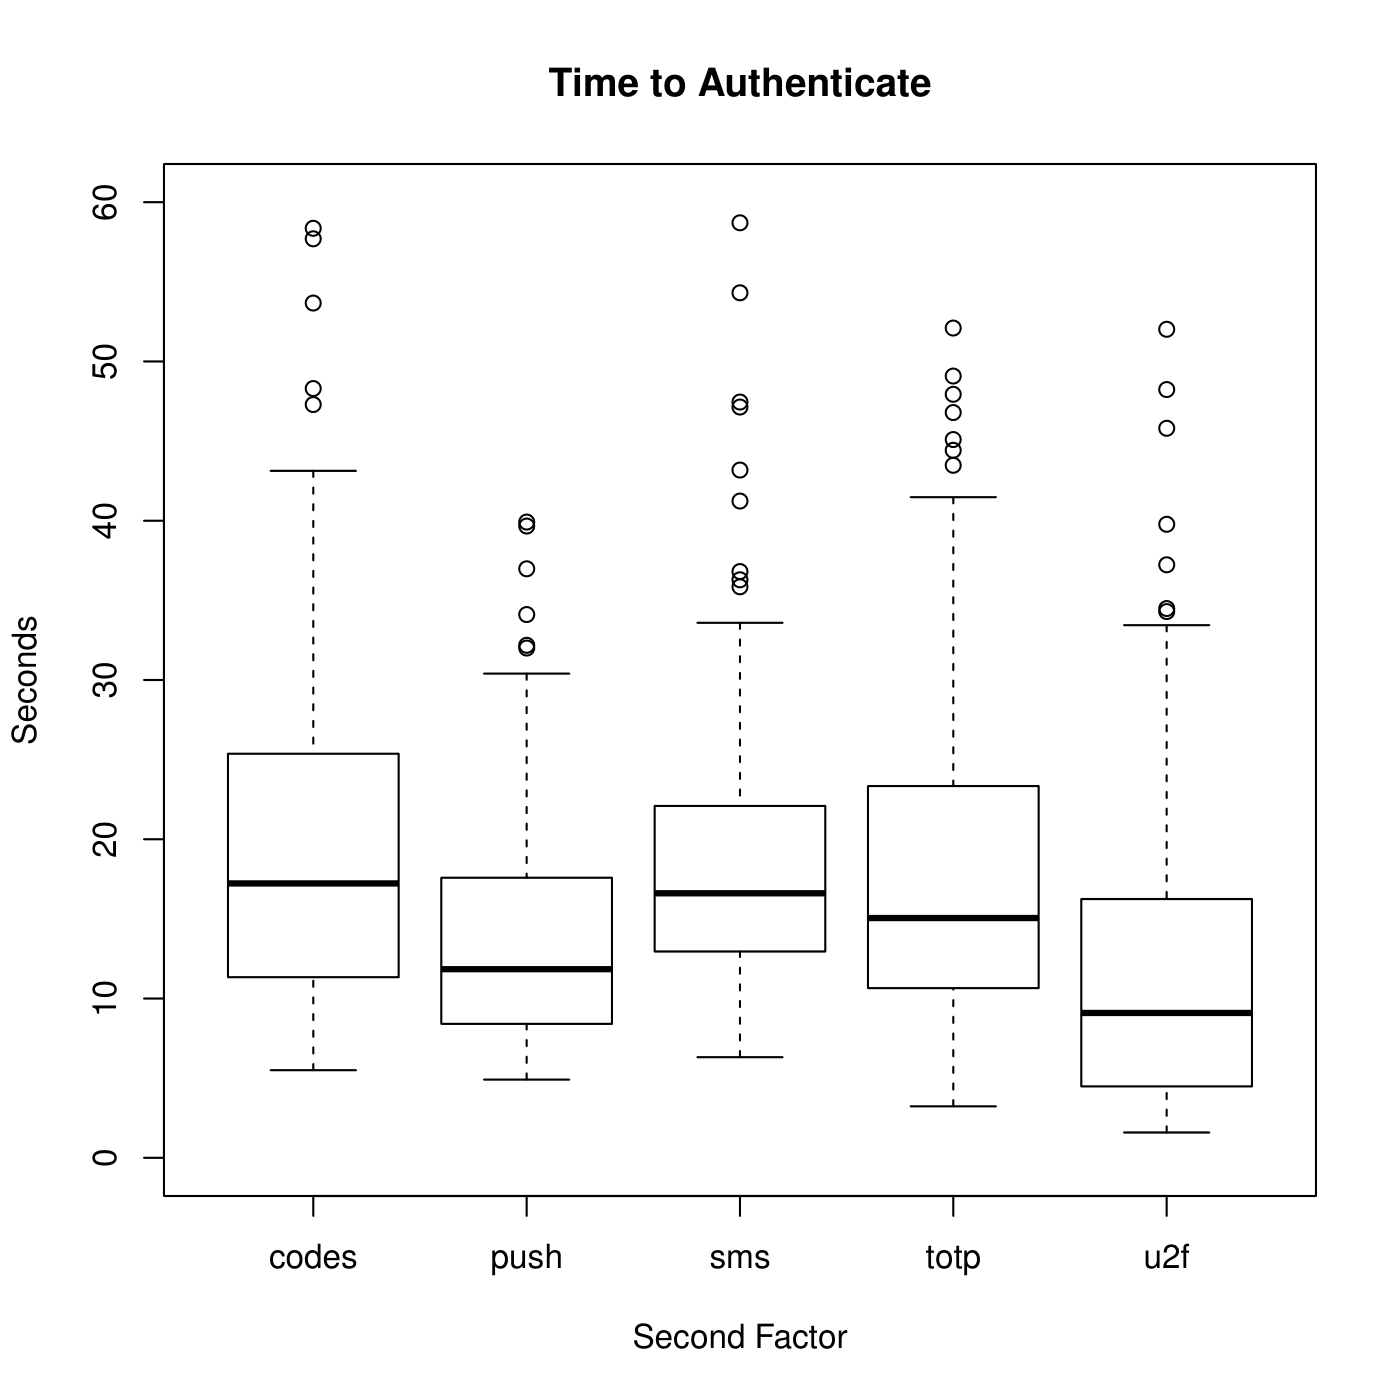
\includegraphics[height=0.8\textheight]{authentication-time}\cite{reese2019}
    \end{figure}

    \note{
        \begin{itemize}
            \item Erste betrachtete Metrik: Authentifizierungszeit
            \item Zeit, für Passwort benötigt nicht mit eingerechnet
            \item U2F am schnellsten, wahrscheinlich weil Nutzer YubiKey am Gerät stecken haben
            \item am zweitschnellsten Push-Benachrichtigungen
            \item Andere 3 Methoden: Zeit zum Eintippen der Zahlen benötigt, verlangsamt Prozess
            \item SMS: Zeit zum Versenden kommt dazu % chktex 13
            \item Cides müssen rausgesucht werden, nicht unbedingt immer zur Hand
            \item \begin{itemize}
                      \item[\textrightarrow] wahrscheinlich große Varianz aufgrund von verschiedenen Aufbewahrungsmöglichkeiten
                  \end{itemize}
        \end{itemize}
    }

\end{frame}

\begin{frame}
    \frametitle{Gebrauchstauglichkeit der Authentifizierung}

    \begin{itemize}
        \item Bewertung der wahrgenommenen Gebrauchstauglichkeit nach der Standardskala SUS\,
\includegraphics[height=0.25\baselineskip]{sus}
              {\tiny\textcolor{white}{\endnote{\url{https://borderpolar.com/wp-content/uploads/2021/06/red-among-us-png-842x1024.png.webp}}}} % chktex 29
    \end{itemize}
    \begin{figure}[c]
        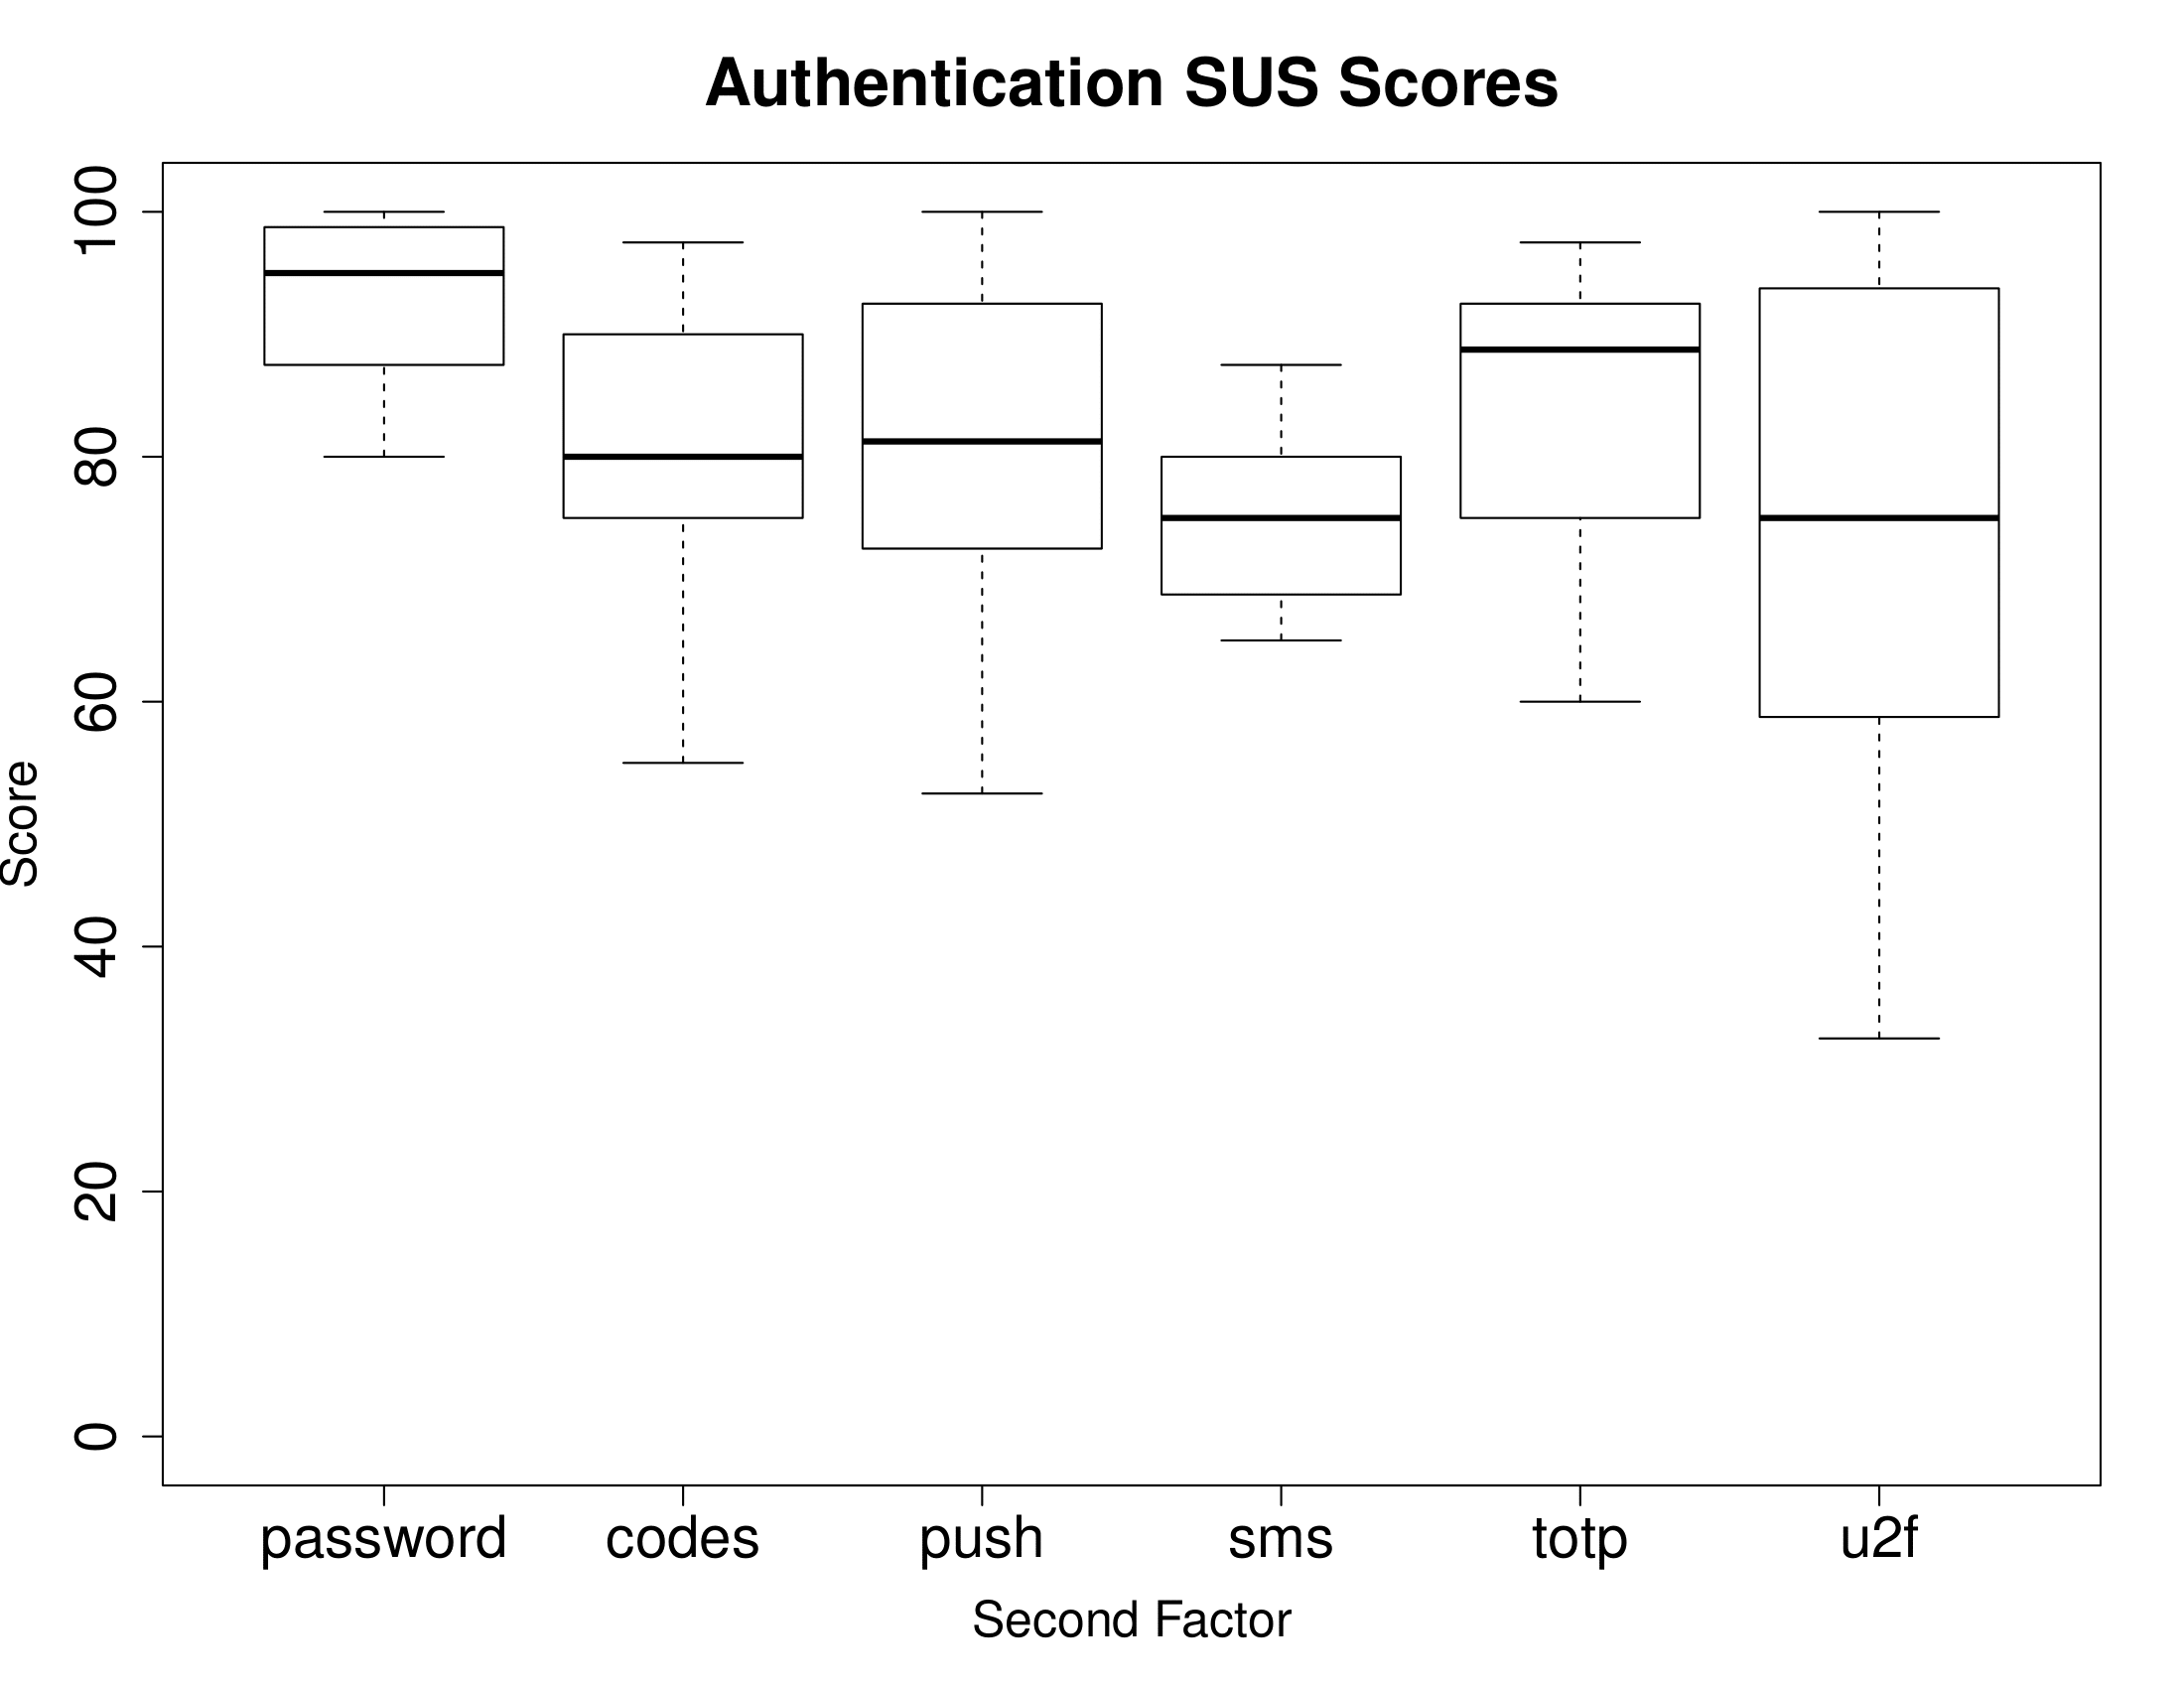
\includegraphics[height=0.76\textheight]{authentication-sus}\cite{reese2019}
    \end{figure}

    \note{
        \begin{itemize}
            \item Passwort als Kontrollwert
            \item andere Werte alle schlechter, fügen ja nur weitere Schritte hinzu
            \item obwohl TOTP am drittlangsamsten, höchster Score unter 2FA-Methoden
                  \begin{itemize}
                      \item Google App wurde benutzt, Implementierung wahrscheinlich nutzerfreundlich
                      \item Manche Personen haben sich beschwert, dass die Codes zu schnell ablaufen zum Eingeben
                      \item Erklärt auch längere Zeit aus vorheriger Folie
                  \end{itemize}
            \item Auch interessant: U2F hatte sehr große Varianz, schnitt am schlechtesten ab, obwohl zeitlich am schnellsten
                  \begin{itemize}
                      \item Zeit nicht alles, muss auch komfortabel sein
                      \item große Unterschiede durch verschiedene Möglichkeiten YubiKey aufzubewahren
                      \item[\textrightarrow] nicht alle wollen extra Gerät, ist kein Handy was man so oder so hat
                  \end{itemize}
        \end{itemize}
    }

\end{frame}

\subsection{Einrichtung von 2FA}
\begin{frame}
    \frametitle{\currentsectionname}

    \begin{itemize}
        \item Einrichtung der fünf verschiedenen 2FA-Methoden wurde betrachtet
        \item gezielte getrennte Betrachtung von der generellen Gebrauchstauglichkeit
        \item 30 Teilnehmer*innen, welche jeweils jede Methode einrichten mussten
    \end{itemize}

    \note{
        \begin{itemize}
            \item getrennte Betrachtung, damit schlechte Einrichtungserfahrung restliche Einschätzung nicht verfälscht
            \item falls eigentliche Gebrauchstauglichkeit gut ist, nimmt man vielleicht eher eine schlechte Einrichtung in Kauf
            \item Außerdem kann beides getrennt voneinander verbessert werden
        \end{itemize}
    }

\end{frame}

\begin{frame}
    \frametitle{Einrichtungszeit}

    \begin{itemize}
        \item Zeit zwischen Beginn der Einrichtungsaufgabe bis zur Fertigstellung
    \end{itemize}
    \begin{figure}[c]
        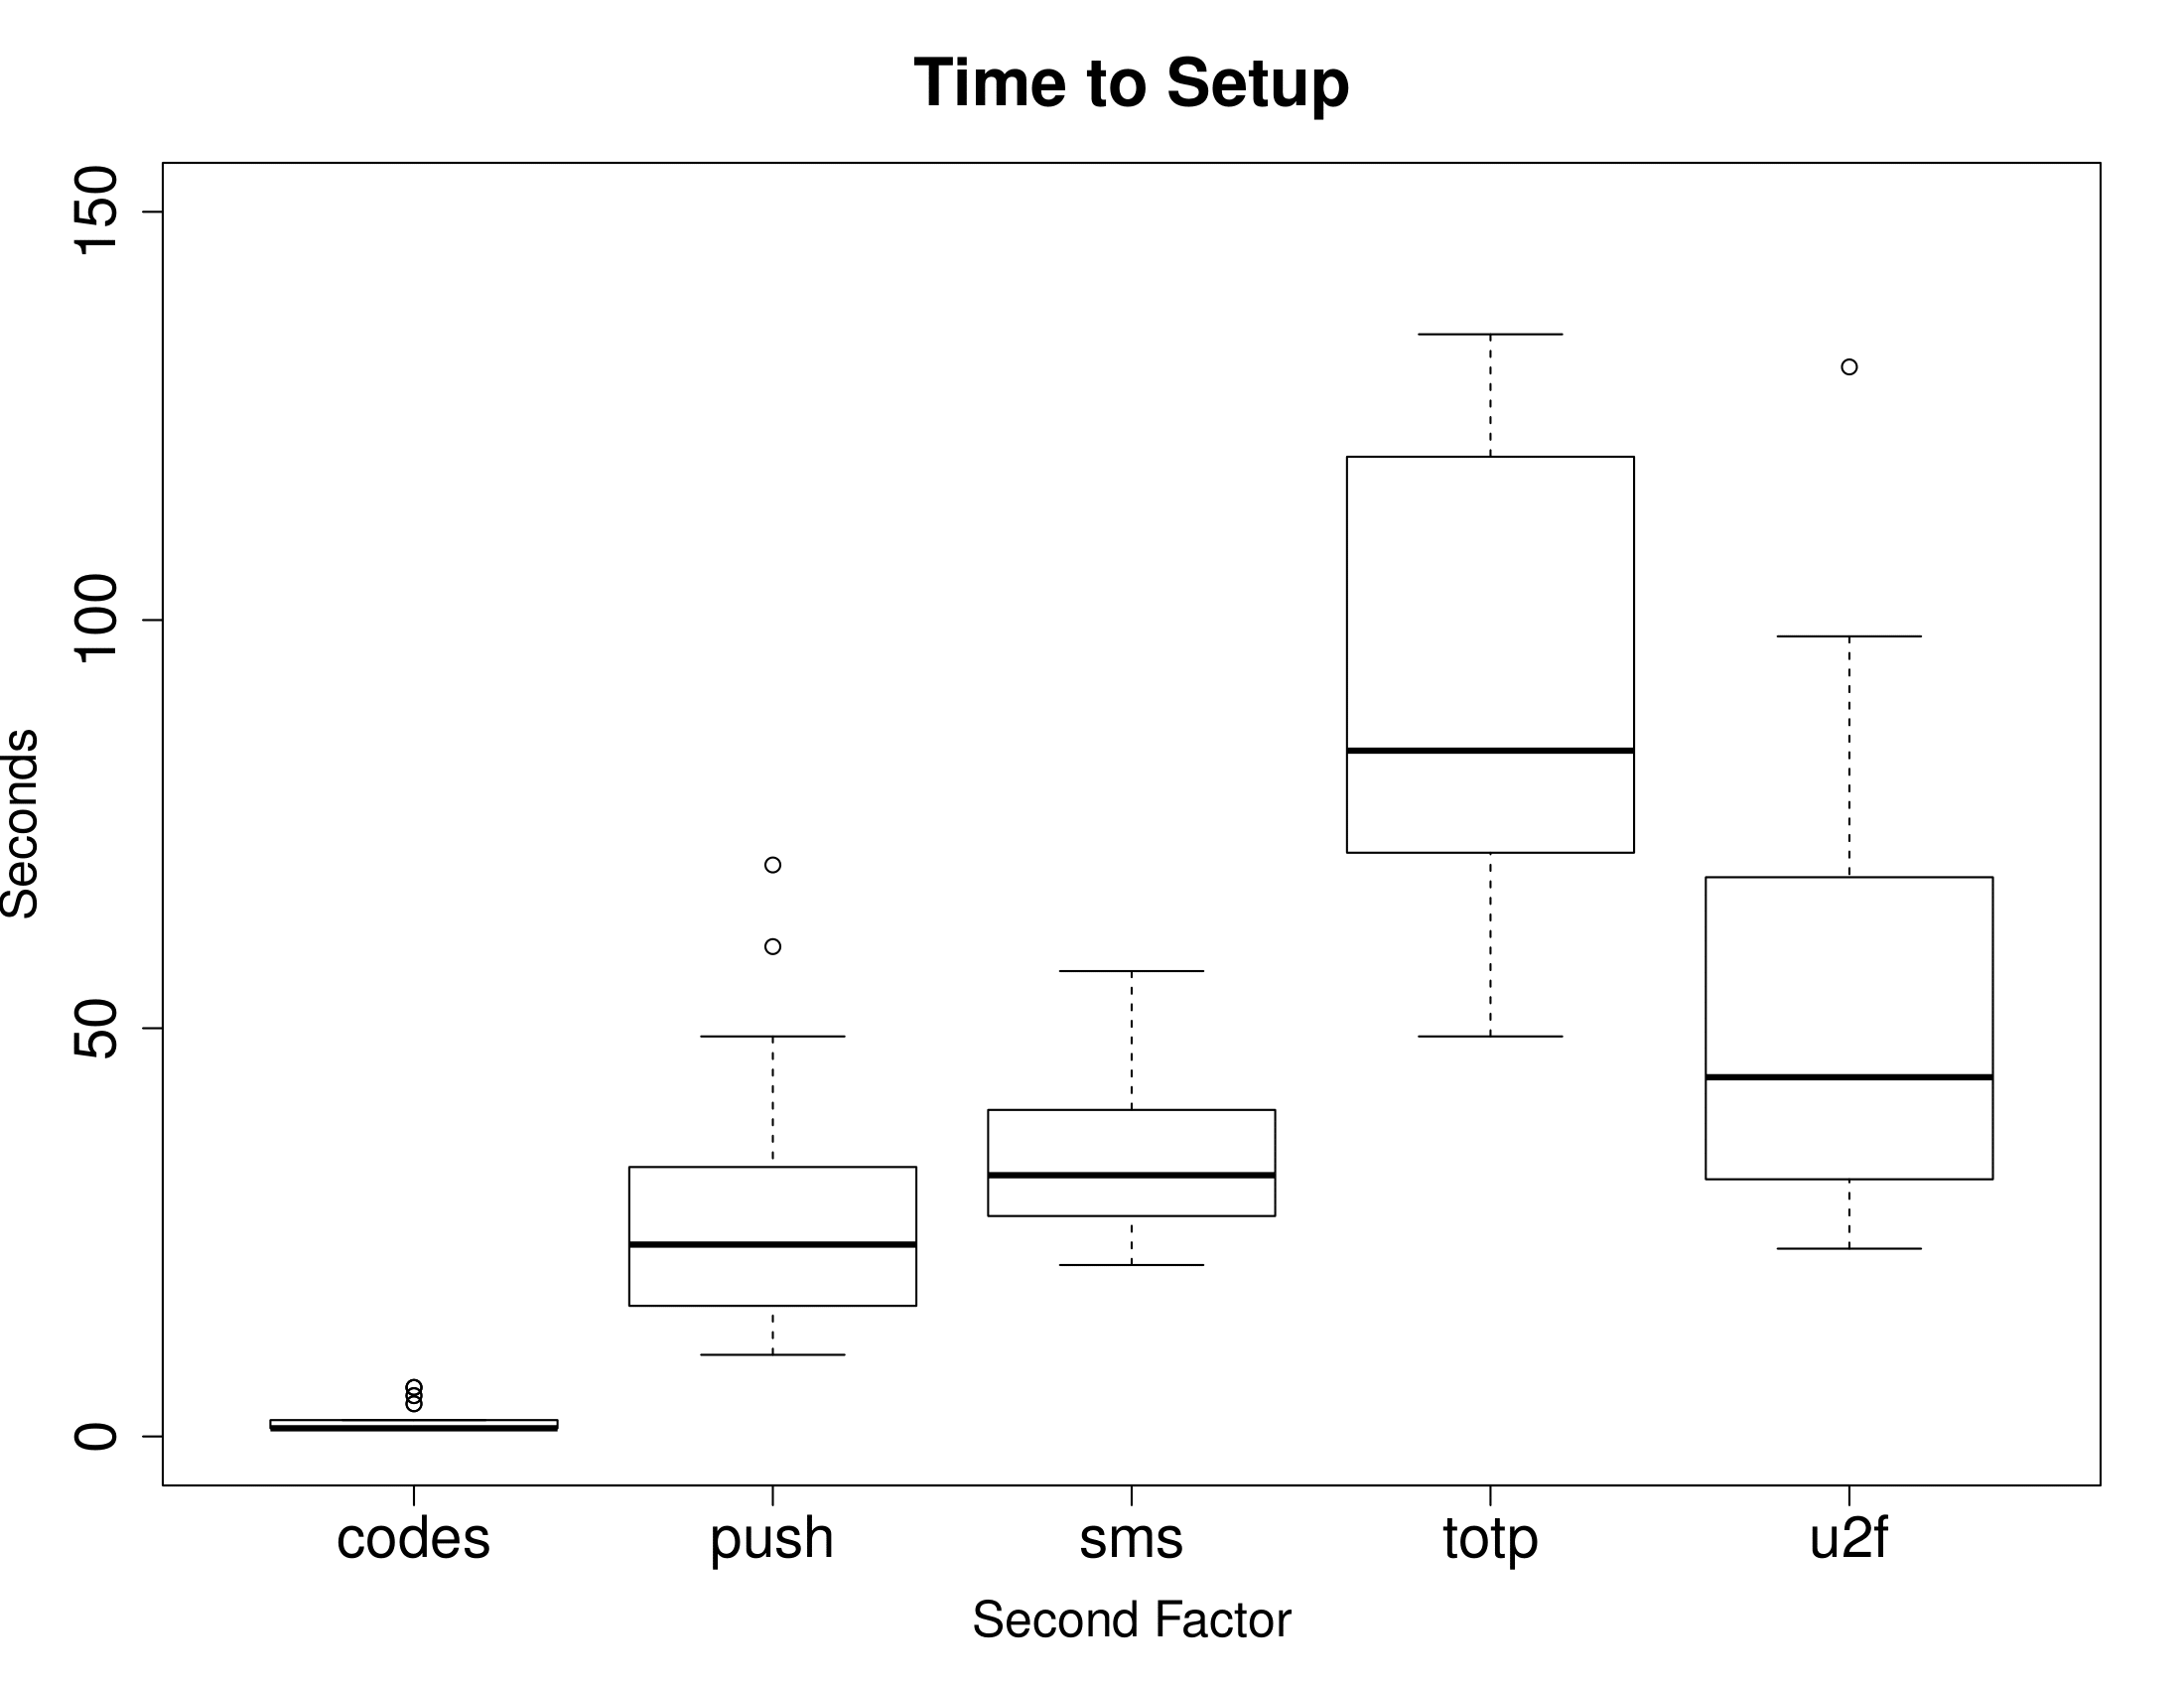
\includegraphics[height=0.8\textheight]{setup-time}\cite{reese2019}
    \end{figure}

    \note{
        \begin{itemize}
            \item Einrichtungszeit für Codes am geringsten,
                da Zeit zum Abspeichern / Ausdrucken / wie auch immer aufbewahren nicht mit betrachtet wurde
            \begin{itemize}
                \item[\textrightarrow] Zeiten wären zu unterschiedlich voneinander gewesen, da schon von Drucker abhängt
            \end{itemize}
            \item Push und SMS am zweitschnellsten, Angabe von Telefonnummer und Verbindung mit Push-App schnell
            \item TOTP und U2F hatten zwei fehlgeschlagene Einrichtungen und waren am langsamsten
            \item Langsame Einrichtung von U2F trotzdem noch bei ca.\ einer Minute
            \begin{itemize}
                \item[\textrightarrow] durch schnelle tagtägliche Benutzung vielleicht zu Entschuldigen
                \item Allerdings muss Nutzer bereits U2F Gerät wie YubiKey besitzen
            \end{itemize}
        \end{itemize}
    }

\end{frame}

\begin{frame}
    \frametitle{Gebrauchstauglichkeit der Einrichtung}

    \begin{itemize}
        \item Erfassung über Single Ease Question (SEQ), Skala von 1 bis 7
    \end{itemize}
    \begin{figure}[c]
        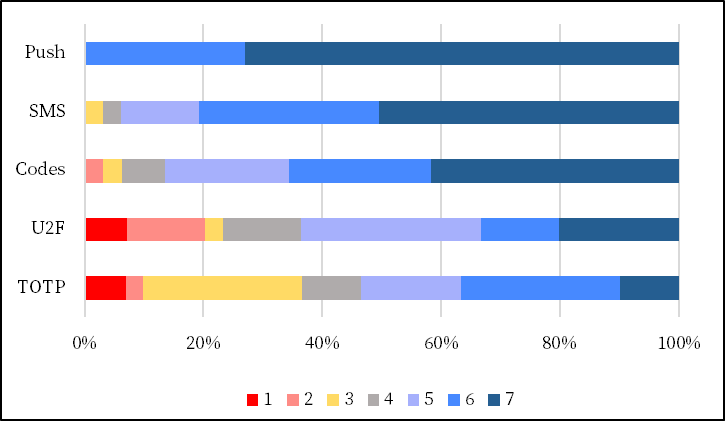
\includegraphics[height=0.7\textheight]{setup-seq}~\cite{reese2019}
    \end{figure}

    \note{
        \begin{itemize}
            \item Nutzer bewerten Usability über Single Ease Question
            \begin{itemize}
                \item Eine Frage: ``Wie Einfach war es, die Einrichtung abzuschließen?''
                \item Bewertung auf Skala von 1 bis 7, von sehr schwer bis sehr einfach
                \item Wahl von SEQ, um Ermüdung vorzubeugen, da alle Teilnehmer*innen alle Methoden eingerichtet haben
            \end{itemize}
            \item mit zeitlicher Erfassung übereinstimmend Push und SMS am einfachsten eingestuft
            \item Vermutung:
            \begin{itemize}
                \item Bekannheit von SMS verbessert Ergebnis von SMS
                \item die meisten kennen U2F und TOTP nicht, weshalb die Scores schlechter sein könnten
            \end{itemize}
        \end{itemize}
    }

\end{frame}
